\section{Vehicle description}
The technology which has been provided for the prototype is a tracked vehicle, seen on \figref{TrackedVehicle}. A platform of the same size of the vehicle  is mounted on the vehicle to protect the mechanical system and to support the system, which include PCB boards, the battery, and the sensors used to control the vehicle. When the platform is mounted on, the vehicle is 45 cm long, 29 cm in width, 12 cm in height and it weighs 2932 grams.\\
The testing will take place in Aalborg University Vicon Room, where the GoT system is installed and calibrated with the appurtenant transmitter, which is mounted on the tracked vehicle during test.

\begin{figure}[H]
	\centering
	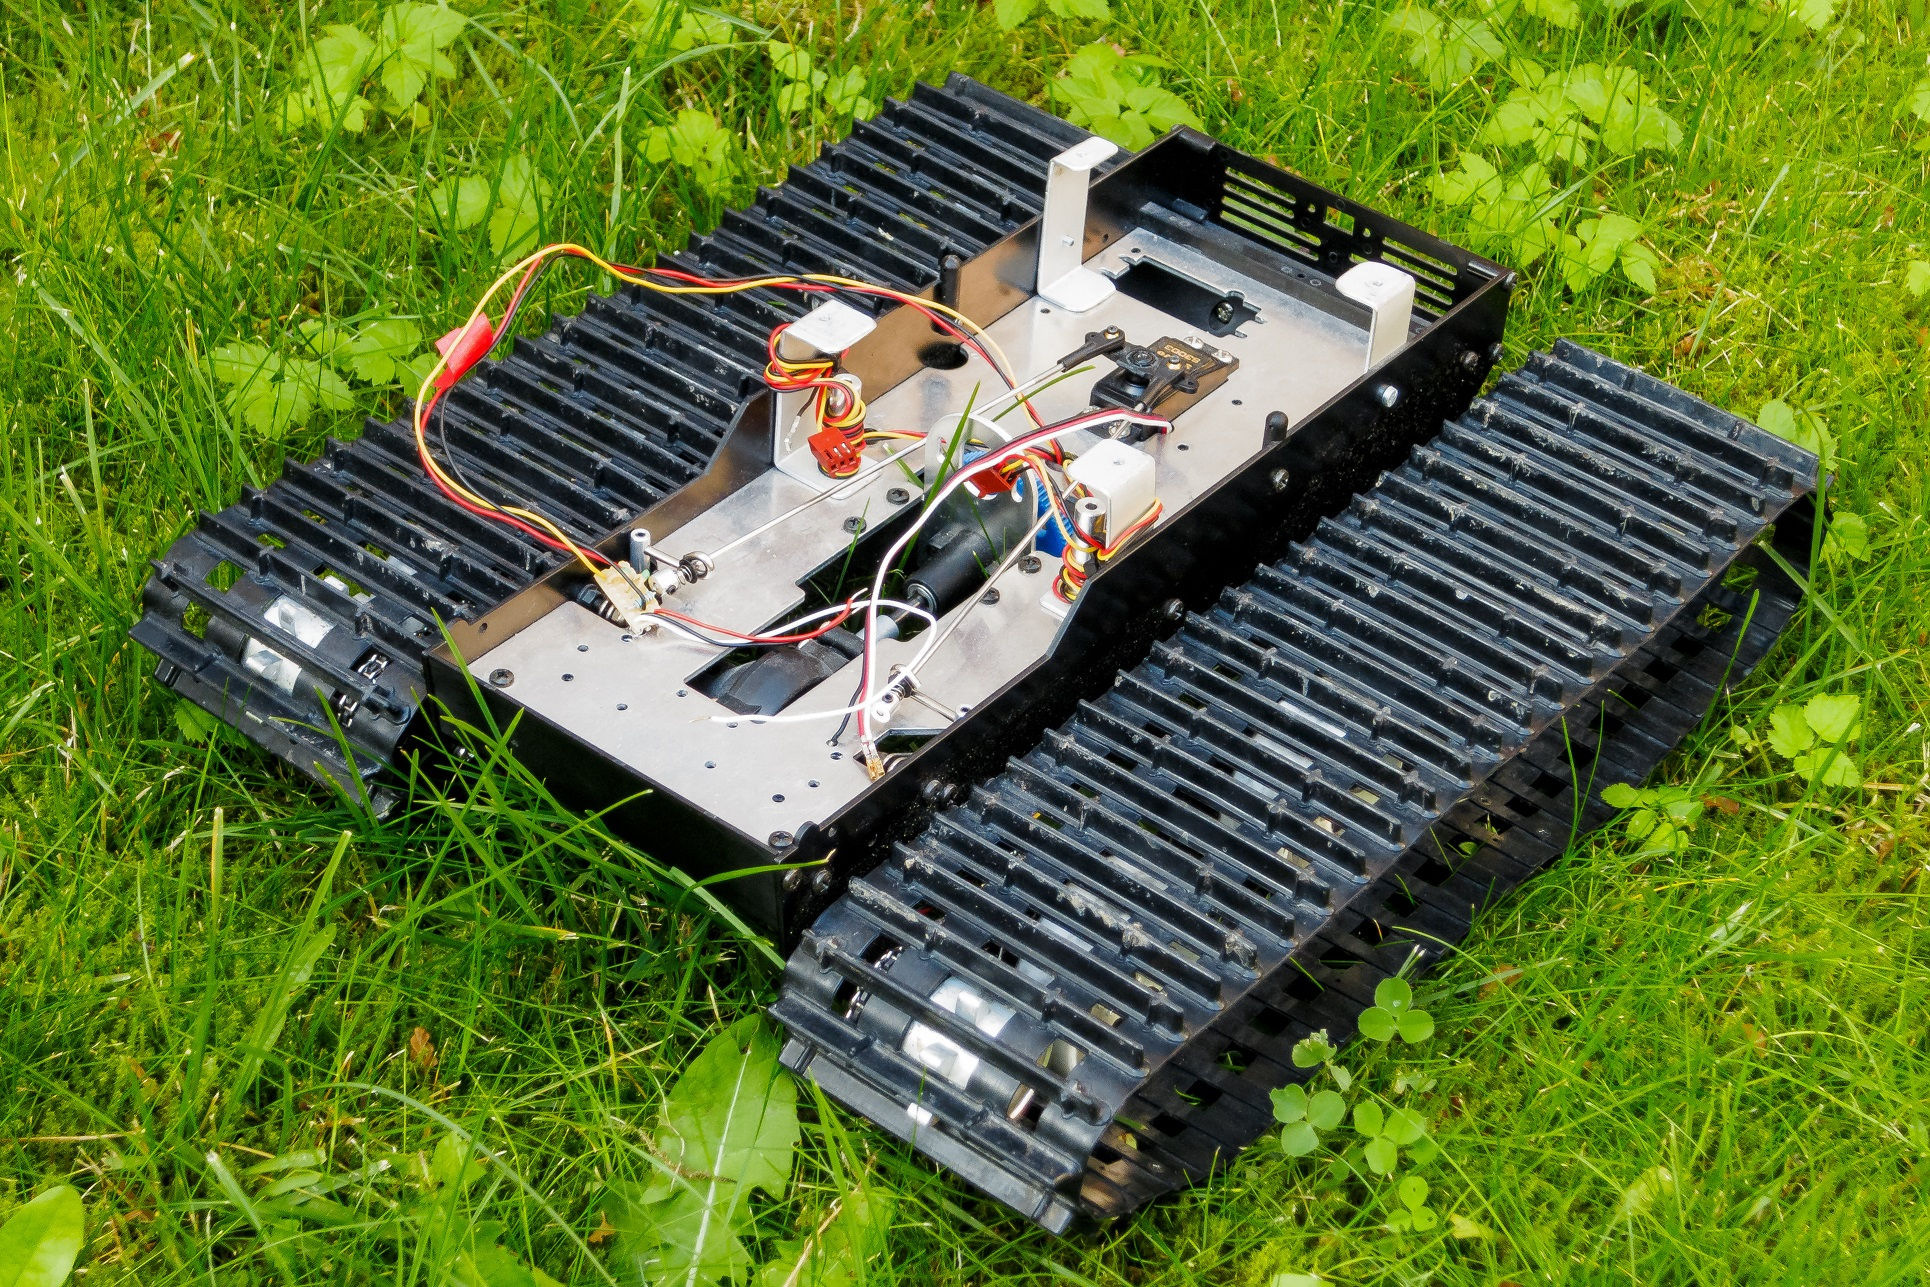
\includegraphics[scale=0.8]{figures/BeltVehicle.jpg}
	\caption{The provided track vehicle}
	\label{TrackedVehicle}
\end{figure}

\todo{datasheet of the vehicle}

The following sections will analyse the vehicle mechanical system, and the features that the vehicle use to drive and steer.

\subsection{Drivetrain}

The drivetrain of a motored vehicle, is the components that transfer the rotational energy from the motor to the driving wheel of the vehicle. For this vehicle, the drivetrain will contain the gear connected to the brushed DC motor, the differential gear box and the gears connected to the belts. The drivetrain is shown on \figref{vehicleDescriptionDriveTrain}.

\begin{figure}[H]
	\centering
	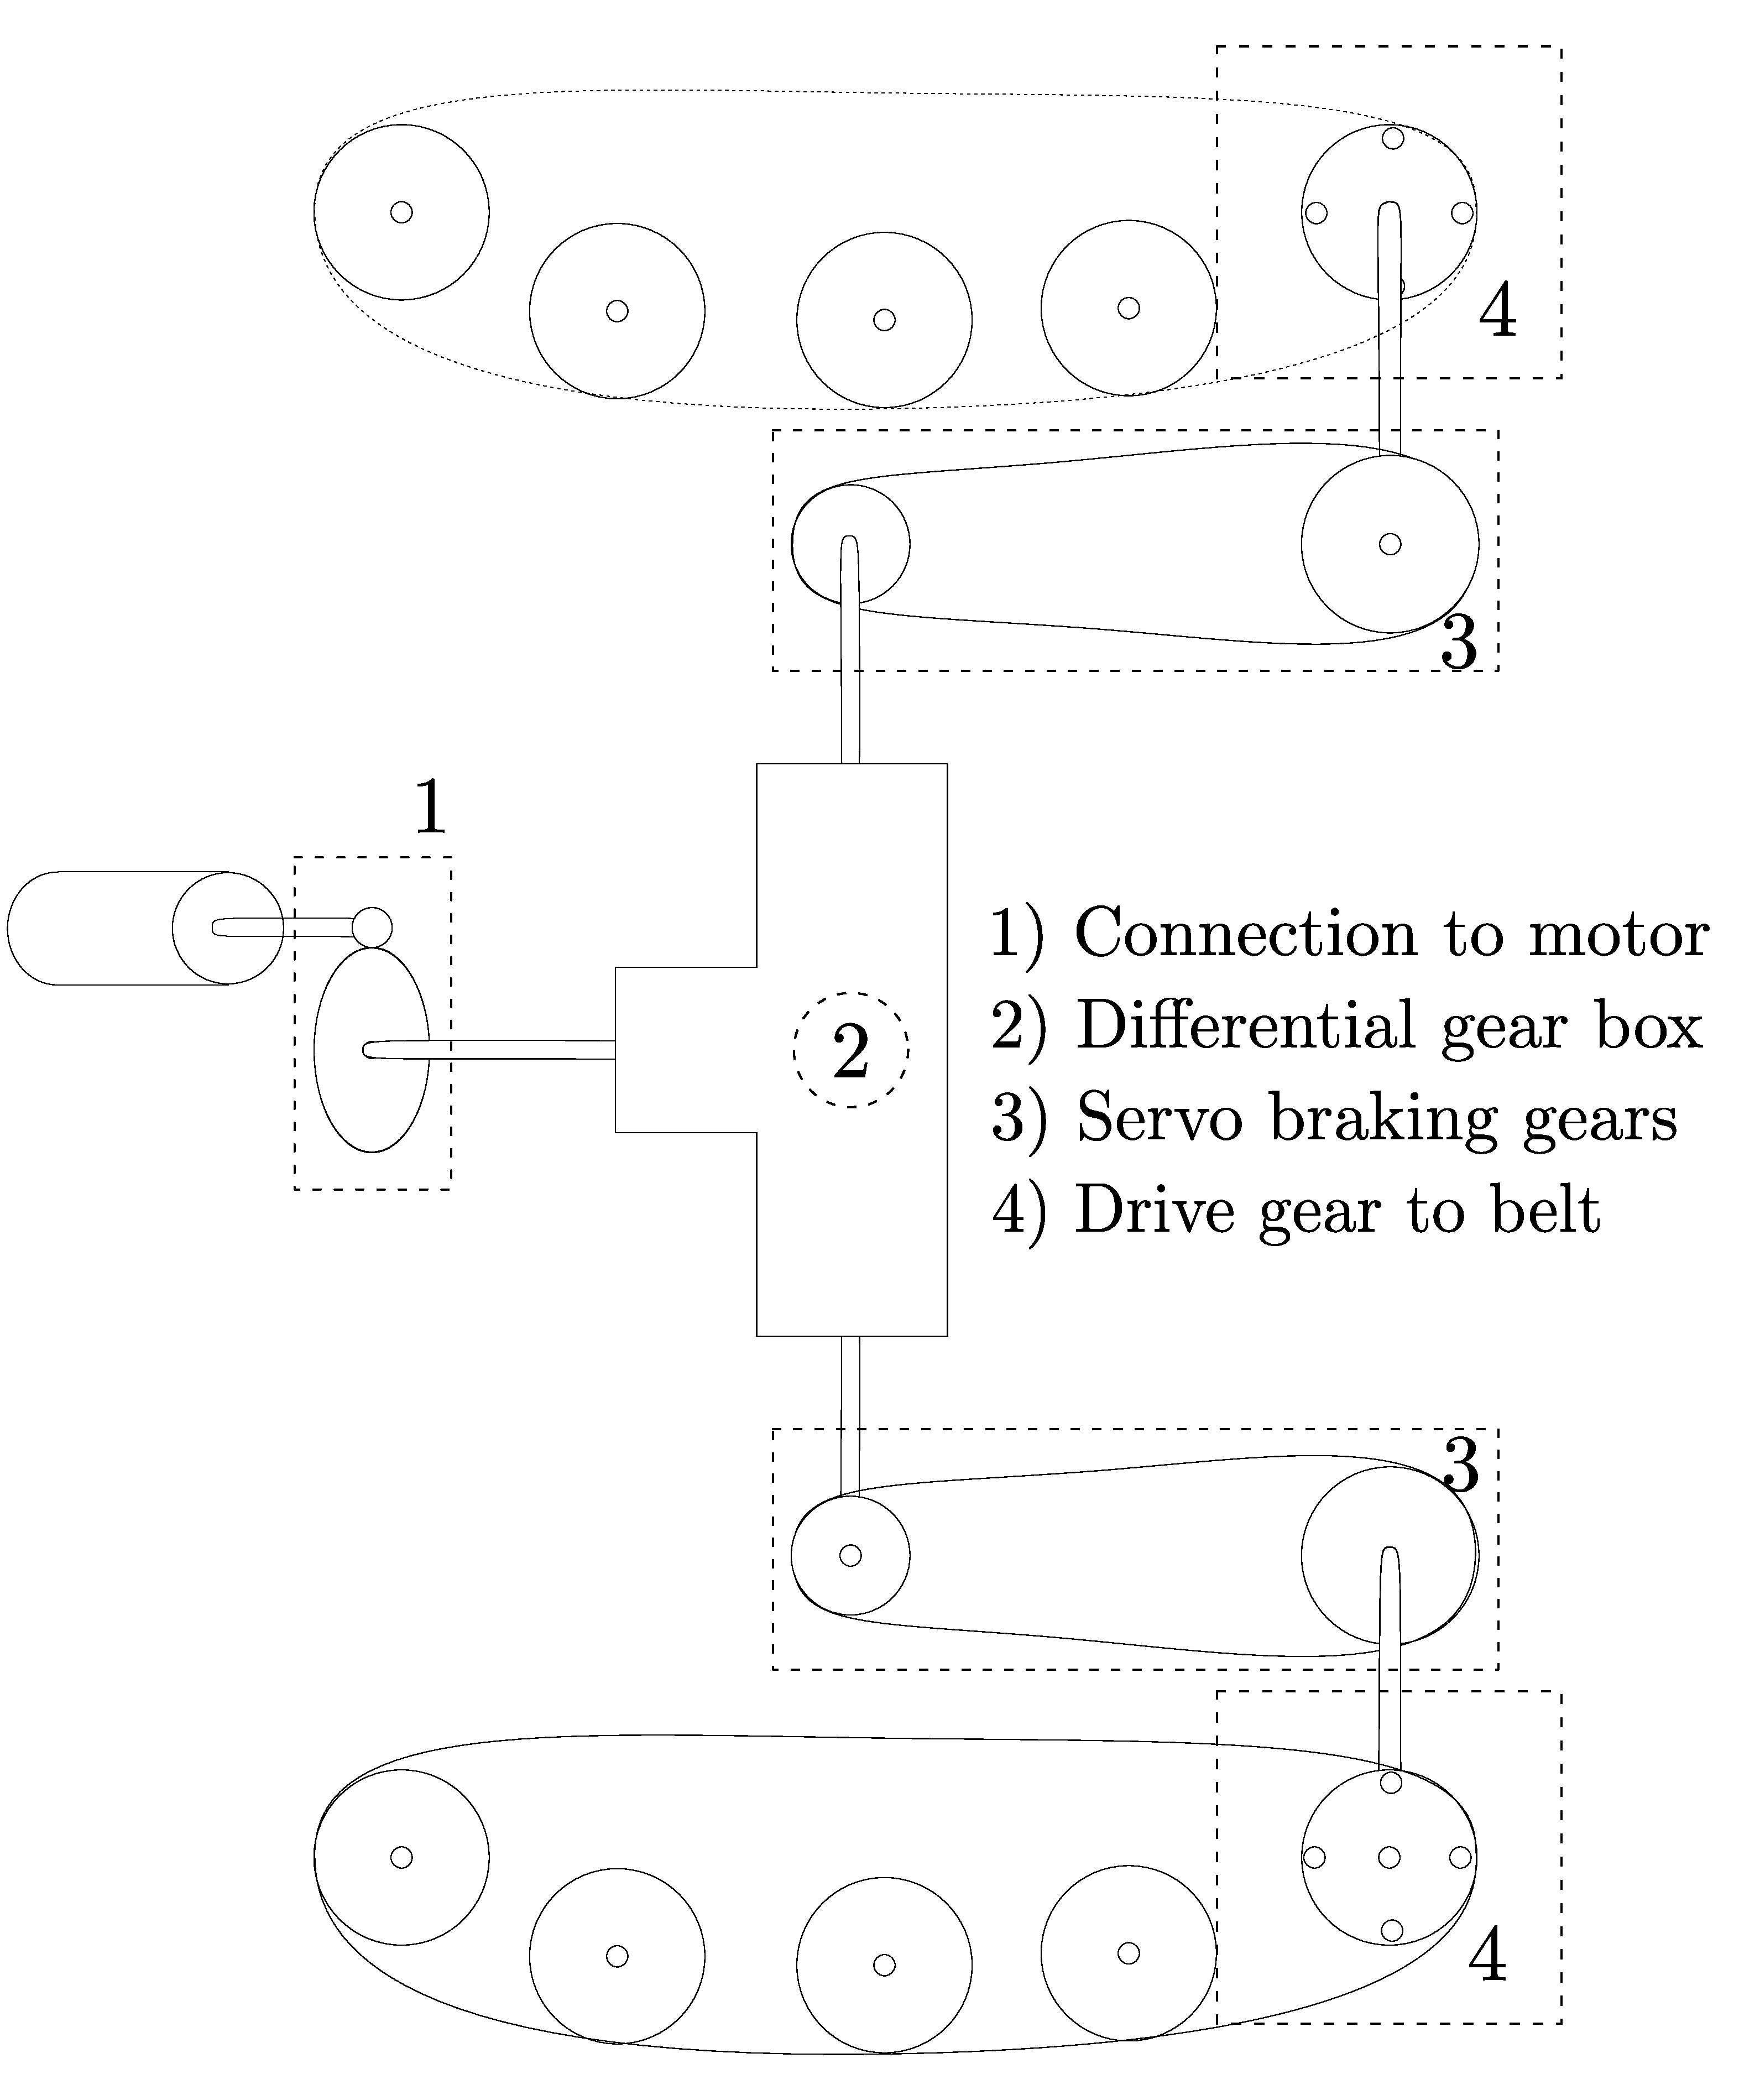
\includegraphics[scale=0.2]{figures/vehicleDescriptionDriveTrain.pdf}
	\caption{Illustration of the drive train of the vehicle.}
	\label{vehicleDescriptionDriveTrain}
\end{figure}

The motor apply a force to the system at the start of the drivetrain(1). The differential gear box(2) is direclty connected to the motor. The servo controls the steering, by applying a breaking force on the breaking gears(3). The rotational power is then transmitted to the other track through the differential gear box(2). The vehicle runs on two belts, that envelop on each side 4 free wheels, plus a gear wheel connected to the drivetrain(4). A Hall sensor is setup on each gear wheel(4), to measure the speed of each belt.\\
The following sections will describe the different parts of the drivetrain seen on \figref {vehicleDescriptionDriveTrain}.\\